\chapter{Teoretski uvod}
\label{chap:teoretski-uvod}

\section{Homologija proteina}
\label{sec:homologija}

Homologija u biološkom smislu predstavlja slične osobine među vrstama na
različitim razinama organizacije života, poput organa, tkiva, stnice ili
molekule. Homologne osobine uočene među jedinkama različitih vrsta obično
upućuju na zajedničke pretke tih vrsta u evoluciji. Međutim, u molekularnoj
biologiji termin homolog se često koristi i za naznačavanje sličnosti. bez
obzira na genetsko srodstvo.\cite{bioinfo1}

\begin{figure}[h!]
\centering
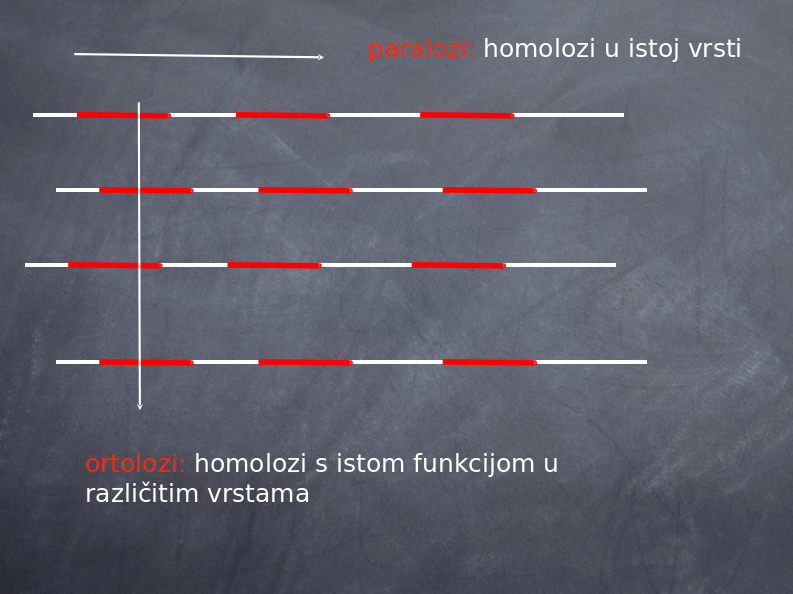
\includegraphics[width=4.5in]{figures/ortho-para.png}
\caption{Vizualni prikaz ortolognih i paralognih gena na genetskim lancima
raznih vrsta}
\label{fig:para-ortho}
\end{figure}

Za homologne sekvence proteina kažemo da su ortologne kad su direktni
potomci neke sekvence u zajedničkom pretku, bez da su prošle duplikaciju
gena. Drugim riječima, ortologne sekvence se mogu naći u jedinkama
različitih vrsta, a obavljaju istu funkciju u svim tim vrstama. Paralogne
sekvence su homologne sekvence koje su nastale od dvije različite kopije
nekog gena koji je prošao kroz proces duplikacije gena u nekom zajedničkom
evolucijskom pretku. Paralozi se mogu naći u jedinkama jedne ili više vrsta te
ne obavljaju nužno identične funkcije. Slika \ref{fig:para-ortho} predočuje
razliku paraloga i ortologa.



